\section{Detailed design}

The following section will go in to the detail of the design of the different
components in the architecture of \pman. The detailed design will include the
different interfaces (at function level) and the different structures that the
components will implement.

One should bare in mind that even though C does not support the object oriented
paradigm, the detailed design will be depicted with class diagrams. In the
actual implementation the class methods of will be free functions acting on
common data (\texttt{structs}).

\subsection{Database handling}

Database handling is by far the most complex and largest subsystem after
the encryption. This is because secure file based database handling has a lot
of different intricacies not the mention the complex metadata that needs to
be stored. The goal of the design of the database handling subsystem is to
enclose all this in to flexible and easy-to-use interface.

Due to the size of this subsystem, the detailed design is divided in to two
diagrams. One for the database driver and metadata handling, and one for the
entry managing. Lets first see the design of the database driver and metadata
handling in figure \ref{dia:driver_meta}.

\begin{figure}[H]
    \centering
    \centerline{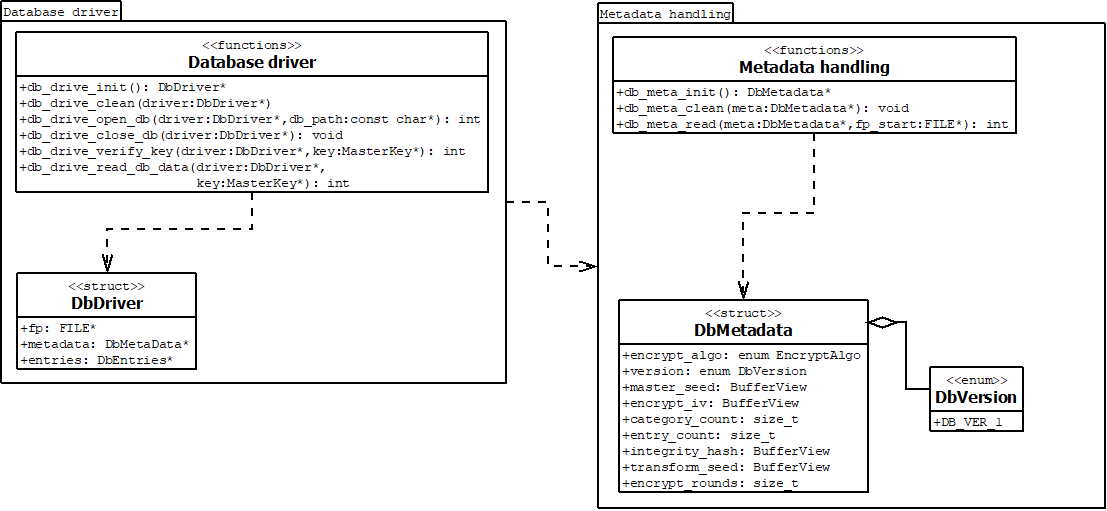
\includegraphics[scale=0.4]{\detaileduml/db_handling/driver_meta}}
    \caption{Detailed design of the database driver and metadata components.}
    \label{dia:driver_meta}
\end{figure}

Bla bla bla

Next, lets view the design of entry manager and line spoof components. This
design is visible in \ref{dia:entry_manage}.

\begin{figure}[H]
    \centering
    \centerline{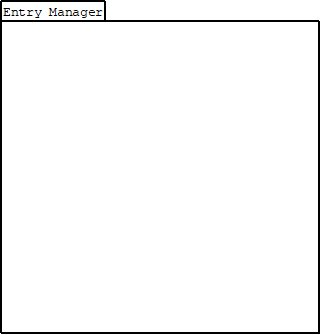
\includegraphics[scale=0.55]{\detaileduml/db_handling/entry_manage}}
    \caption{Detailed design of the entry manager component.}
    \label{dia:entry_manage}
\end{figure}

\subsection{Encryption}

The design of encryption was broken into two parts in the architecture:
File Encryption and Raw Encryption. These two components accommodate the needs
of \pman when it comes to encryption and decryption. The detailed design of
these two components can be seen in figure \ref{dia:encrypt_design}.

\begin{figure}[H]
    \centering
    \centerline{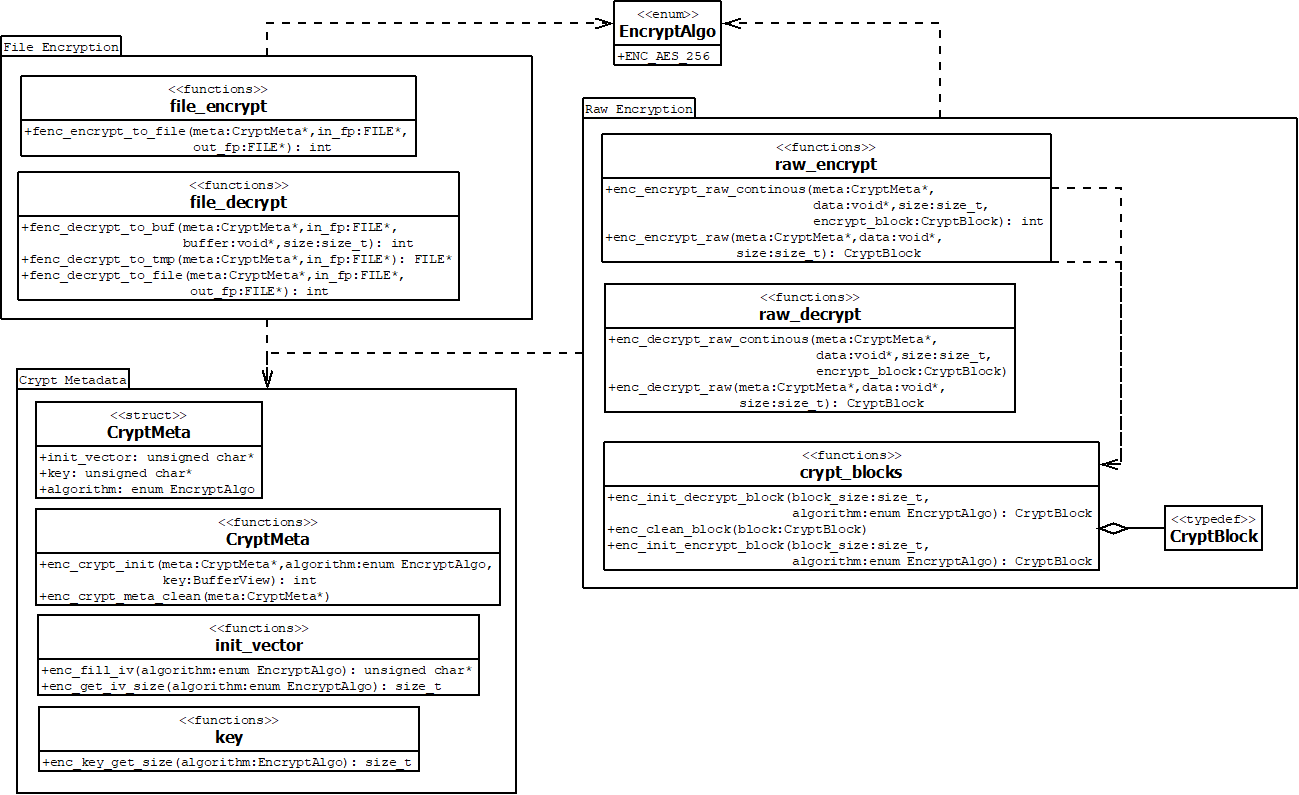
\includegraphics[scale=0.4]{\detaileduml/encrypt/encrypt}}
    \caption{Interfaces and design of the encryption components}
    \label{dia:encrypt_design}
\end{figure}

The class diagrams of figure \ref{dia:encrypt_design} show that the file
encryption side offers quite a minimal interface compared to the raw encryption
side. This is because data encryption itself holds a lot of implementation
details (initialization vectors, different block sizes etc.) that need not to
be revealed when all the user wants to do is encrypt or decrypt a file.

The basic idea of the design is that the user provides the password database
(file) that he wants to encrypt, algorithm and the key that will be used. From
here the implementation will construct the \texttt{CryptMeta} object that is
used with the raw encryption functions, which will contain the key, the
initialization vector, and the requested algorithm.

Then, depending on the size of the requested file encryption/decryption
the functions will either construct a reusable \texttt{CryptBlock} with an
optimal size, or use the one-time encrypt/decrypt functions provided by the
interface (continuous and non-continuous). The continuous ones were designed
to accommodate extremely large databases, where constantly allocating and
de-allocating new blocks would not be feasible.

\subsection{Hashing}

Hashing inherits many of the same design aspects from encryption, as the
operations are quite similar with, of course, hashing being quite simpler.
The design of the hashing component can be seen in \ref{dia:hash_design}.

\begin{figure}[H]
    \centering
    \centerline{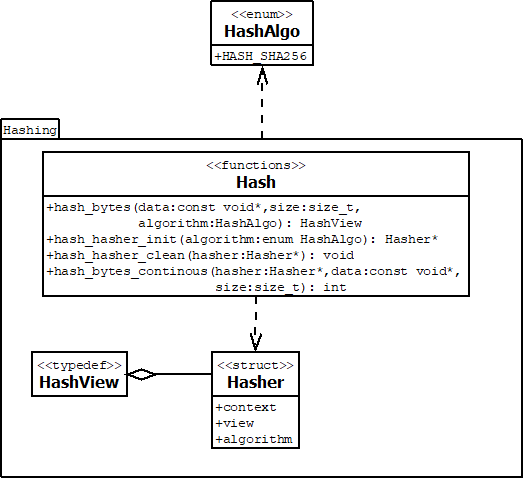
\includegraphics[scale=0.55]{\detaileduml/hash/hash}}
    \caption{Interfaces and design of the hashing component}
    \label{dia:hash_design}
\end{figure}

Both one-time and continuous hashing are supported as with encryption. The user
will either construct a \texttt{Hasher} object to support continuous hashing, or
use the one-time hashing provided with function \texttt{hash\_bytes}.

\subsection{Line spoofing}

\subsection{Authentication}

Compared to a few other components, the purpose and design of authentication is
fairly simply. This is due to it being only an interface that acts as link
between database's and login cache's authentication models. The detailed design
of authentication is visible in \ref{dia:auth_design}

\begin{figure}[H]
    \centering
    \centerline{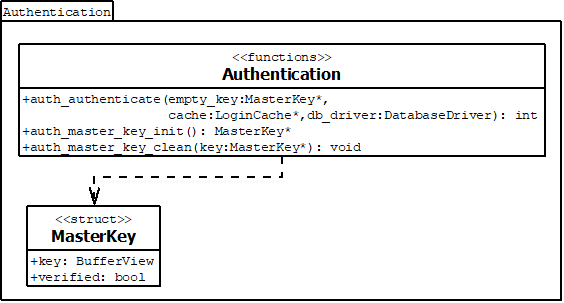
\includegraphics[scale=0.55]{\detaileduml/authentication/authenticate}}
    \caption{Interfaces and design of the authentication component.}
    \label{dia:auth_design}
\end{figure}

As can be seen, the authentication only provides an object which encloses the
master key of the database and provides a unified interface for login cache and
database authentications. The authenticate function should first search the
login cache for any non-expired passwords. If that is not successful it
will prompt the user for the password and validate the password through the
database's methods.

\subsection{Persistence}

The persistance subsystem's job was to handle the login cache and the config
file of \pman. For now, these tasks are quite simple, which is reflected in the
design. The figure \ref{dia:persistence} shows the detailed design of this
subsystem.

\begin{figure}[H]
    \centering
    \centerline{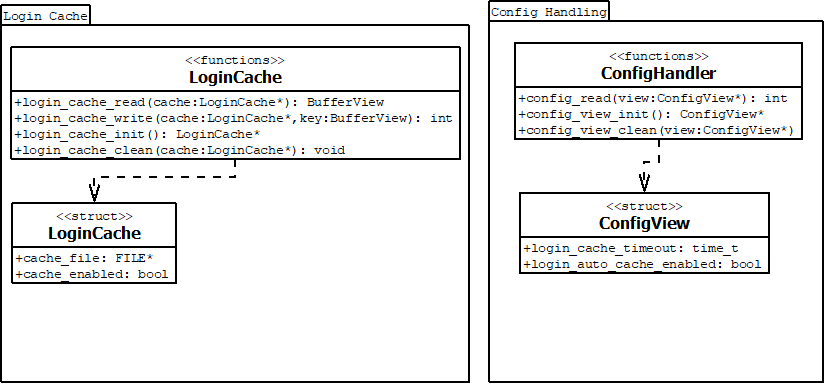
\includegraphics[scale=0.5]{\detaileduml/persistence/persistence}}
    \caption{Interfaces and design of the persistence subsystem.}
    \label{dia:persistence}
\end{figure}

The login cache only handles the storing of the cached master key along with the
time of the expiration. Thus, the \texttt{LoginCache} object only holds the
(possibly) open cache file and information whether or not cache is enabled.

The \texttt{ConfigHandler} on the other hand offers a one-time read interface,
which fills the \texttt{ConfigView} object with the stored configurations. This
way the configurations are stored in memory for as long the user wants without
keeping the file open. In the future this interface is easy to supplement with
write operations for dynamic configuration updating.

\subsection{Options}

The option component was designed to provide a general interface for parsing
options and command, and eventually execute them. The detailed design is visible
in figure \ref{dia:options_design}.

\begin{figure}[H]
    \centering
    \centerline{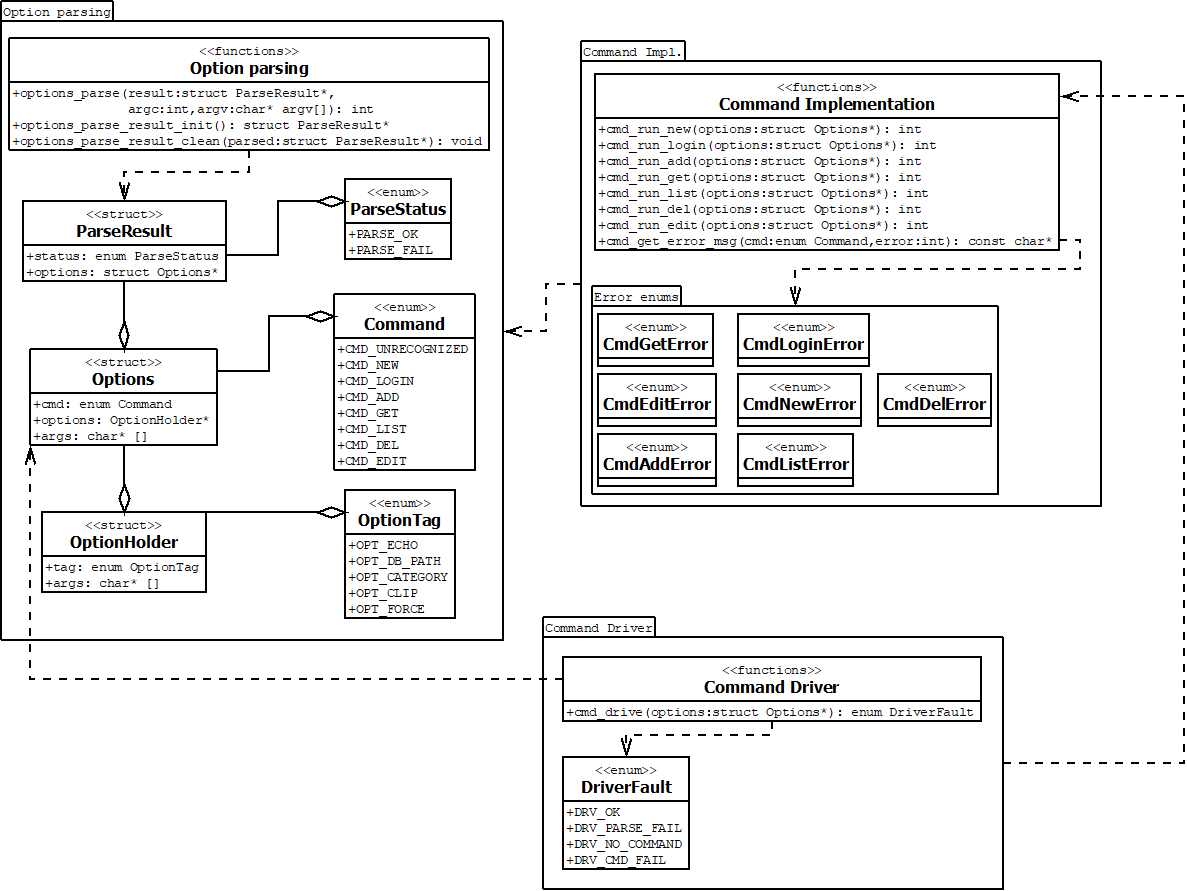
\includegraphics[scale=0.4]{\detaileduml/options/options}}
    \caption{Interfaces and design of the options subsystem}
    \label{dia:options_design}
\end{figure}

The basic idea in the design is to separate parsing, command implementation
and the actual execution of the command. The interfaces here are quite simple
and only provide few functions and error enumerations, which is a good thing.

\subsection{User input}

The user input subsystem provided components for prompts and input validation.
\textbf{Due to time concerns the input validation was dropped, as it is not
priority component.} The figure \ref{dia:prompts_design} shows the detailed
design of the input subsystem.

\begin{figure}[H]
    \centering
    \centerline{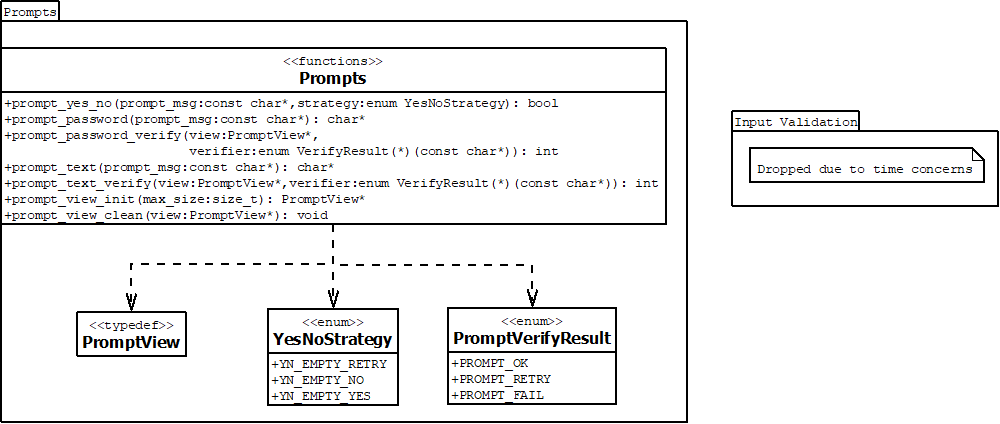
\includegraphics[scale=0.5]{\detaileduml/user_input/input}}
    \caption{Interfaces and design of the input subsystem}
    \label{dia:prompts_design}
\end{figure}

From the design of the prompts component, one can see that the interface offers
both one-time prompts and verified prompts. The verification system works by
a callback interface: the user provides a function that verifies the input and
returns the \texttt{PromptVerifyResult} enumeration. This enumeration is then
used to determine what is done.

The verification system was designed to better facilitate an interface that
can continuously retry the prompt, when the verification fails, or even fail
completely. These kind of verified prompts will see common use among the other
components.

\subsection{Logging}

Again, due to time concerns two of the components in logging subsystem were
left unimplemented. Only the terminal logger was implemented, which is enough
for our use. The figure \ref{dia:logging_design} shows the detailed design of
the logging subsystem.

\begin{figure}[H]
    \centering
    \centerline{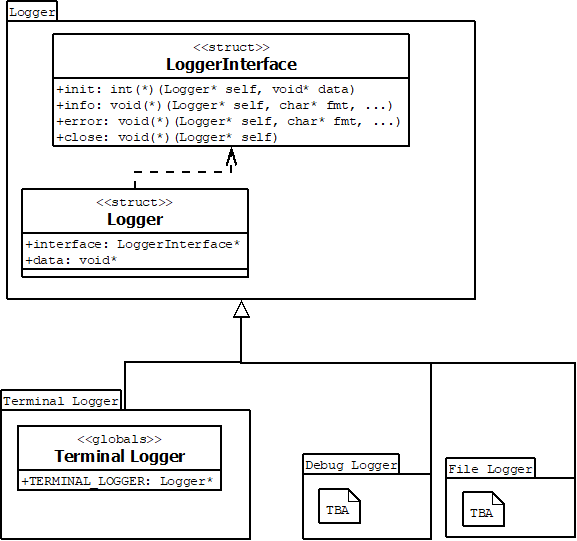
\includegraphics[scale=0.55]{\detaileduml/logging/logging}}
    \caption{Interfaces and design of the logging subsystem}
    \label{dia:logging_design}
\end{figure}

If you are familiar with object oriented practices used in Linux kernel, you
will recognize the OOP pattern used here. Each of the loggers implement a
certain interface (\texttt{struct} of function pointers), which is linked with
each logger object. This way we can pass any type of logger object around the
program (terminal, file or debug logger), and the logging works with that same
interface.
